\section{Matrix-free randomized SVD of the forward operator}
\label{sec:rsvd}

% Source: thesis/sections/3_approximating_the_forward_operator.tex
% \section{Approximating the forward operator}\label{sec:approximating}
\begin{figure*}[thbp]
    \centerline{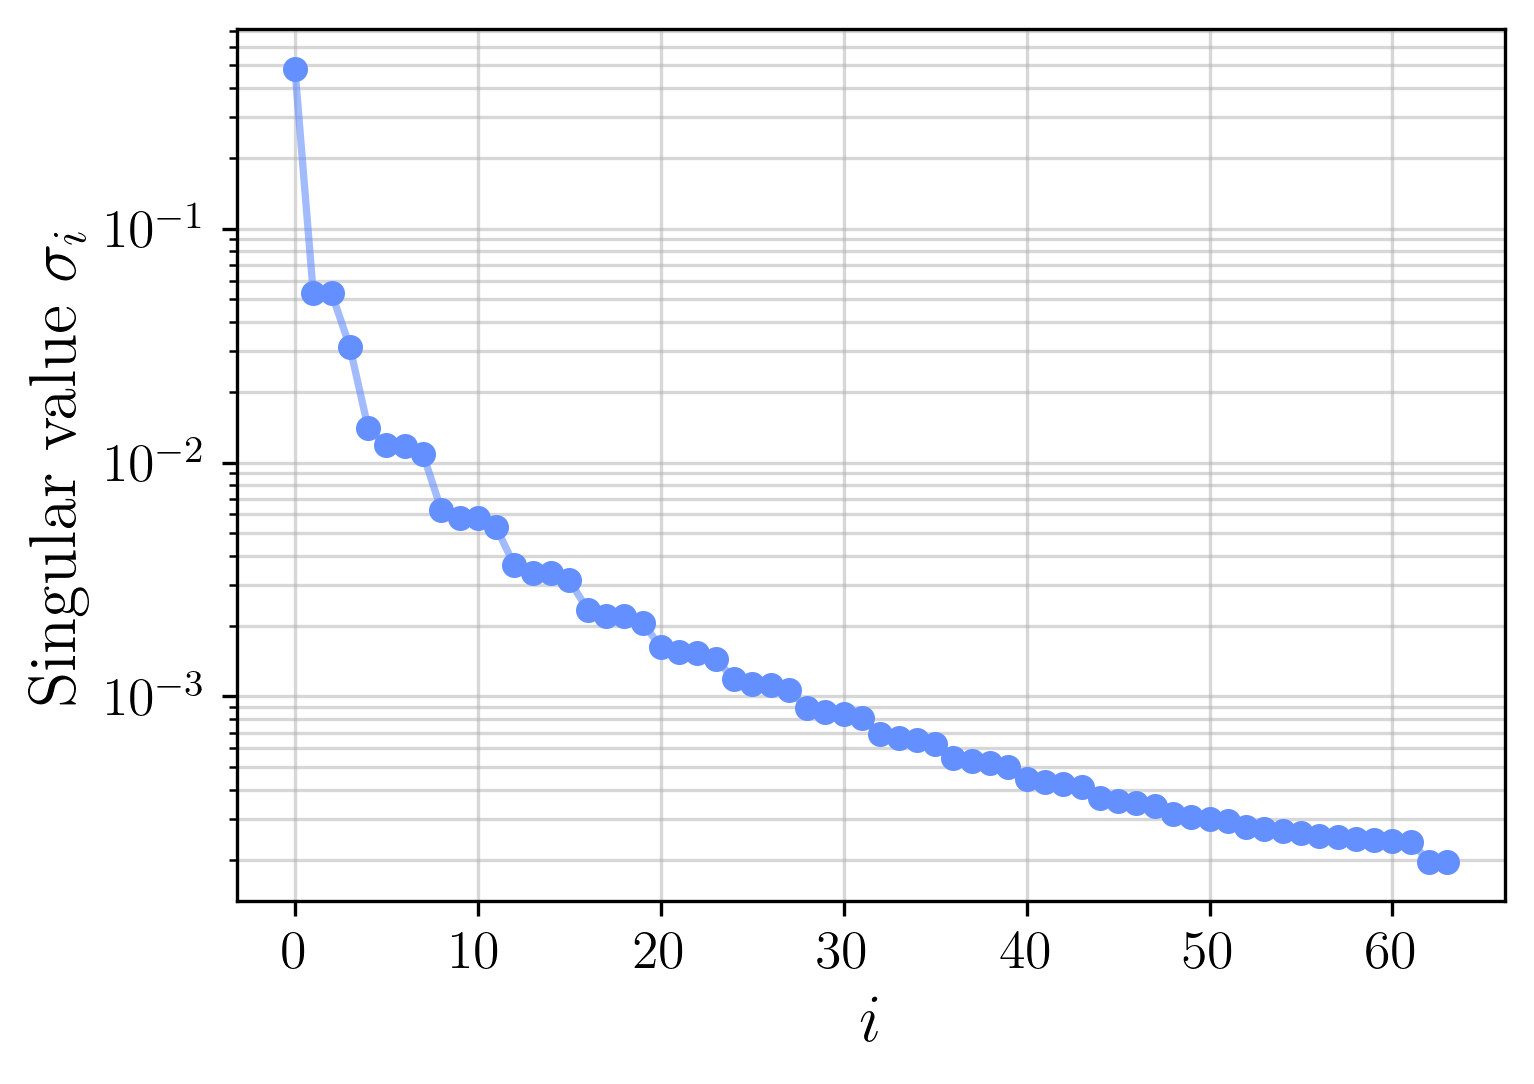
\includegraphics[width=0.6\textwidth]{singular_values.png}}
    \caption{The rapidly decaying singular values $\sigma_1, \dots, \sigma_{64}$ of a $64 \times 289$ matrix $K$ constructed from a $16 \times 16$ rectangular mesh. The y-axis uses a log scale.}
    \label{fig:singular_values}
\end{figure*}
% Opening: motivation and feasibility
The goal of this section is to compute the regularization weights given in Equation \eqref{eq:weights}, which requires the SVD $K = U\Sigma V^T$. Using the identity $K^T = MA_h^{-1}T^T$, $K$ can be formed with $N_b$ linear solves of $A_h v_i = T^T e_i$. With a sparse Cholesky factorization of $A_h$ at cost $\mathcal{O}(N^{3/2})$ and triangular solves at $\mathcal{O}(N \log N)$ in two dimensions (Section~\ref{sec:initial_matrix_factorizations}), forming $K$ takes $\mathcal{O}(N_b N \log N)$. The SVD of the resulting dense $N_b \times N$ matrix then costs $\mathcal{O}(N_b^2 N)$ \cite{dongarraSingularValueDecomposition2018}. Since $N$ grows quadratically with mesh resolution in two dimensions and cubically in three, forming $K$ and computing its SVD is infeasible at fine meshes.

The randomized SVD (Algorithm~\ref{alg:rsvd}) reduces this cost to $\mathcal{O}(l N_b N)$ \cite{halkoFindingStructureRandomness2011}, where $l = k + p$ is a small constant, $k$ is the target rank, and $p$ is an oversampling parameter (typically, $p \in [5, 10]$ \cite{halkoFindingStructureRandomness2011}). It yields a rank-$k$ approximation $K \approx U \Sigma V^T$, and since $K$ has a large nullspace and rapidly decaying singular values, as illustrated in Figure~\ref{fig:singular_values}, $l$ can be chosen much smaller than $N_b$. Unlike $N_b \sim \sqrt{N}$, $l$ can be held constant when the mesh is refined (as shown in Section~\ref{sec:mesh_resolution_effect_on_reconstruction_error}), so the ratio $l / N_b$ shrinks as $N$ increases and the rSVD becomes increasingly advantageous for larger problems.

The rSVD implementation of Algorithm~\ref{alg:rsvd} requires forming $B = Q^T K$, which requires $K$ to be stored as a dense $N_b \times N$ matrix. We instead propose a matrix-free variant without assembling $K$, at a cost of $l$ forward PDE solves and $l$ adjoint PDE solves.


\subsection{A matrix-free rSVD scheme}\label{sec:a_matrix_free_rsvd_scheme}
\begin{figure}[thbp]
    \centering
    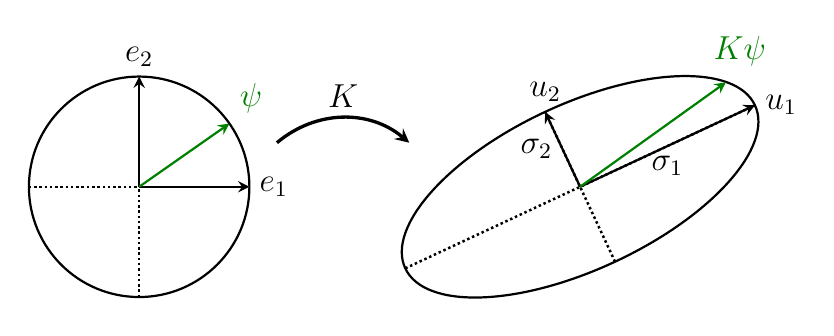
\begin{tikzpicture}[
        scale=0.7,
        >=stealth,
        line width=0.9pt,
        every node/.style={font=\large}
    ]
    % Left: unit circle
    \begin{scope}[shift={(0,0)}]
      % circle
      \draw[thick] (0,0) circle (2);
      % dotted guidelines
      \draw[densely dotted] (-2,0) -- (0,0);
      \draw[densely dotted] (0,-2) -- (0,0);
      % e1, e2
      \draw[thick,->] (0,0) -- (2,0) node[right] {$e_1$};
      \draw[thick,->] (0,0) -- (0,2) node[above] {$e_2$};
      % omega, length=2, angle=35
      \draw[thick,->,Green] (0,0) -- ({2*cos(35)},{2*sin(35)}) node[above right] {$\psi$};
    \end{scope}
    
    % Middle: K arrow
    \begin{scope}[shift={(3.5,0)}]
      \draw[very thick,->]
        (-1,0.8) to[out=40, in=140] (1.4,0.8);
      \node[above] at (0.2,1.25) {$K$};
    \end{scope}
    
    % Right: ellipse + vectors
    \begin{scope}[shift={(8,0)}, rotate=25]
      % ellipse
      \draw[thick] (0,0) ellipse (3.5 and 1.5);
      % dotted principal axes
      \draw[densely dotted] (-3.5,0) -- (3.5,0);
      \draw[densely dotted] (0,-1.5) -- (0,1.5);
      % u1 and u2
      \draw[thick,->] (0,0) -- (3.5,0)
        node[midway, below] {$\sigma_1$}
        node[right] {$u_1$};
      \draw[thick,->] (0,0) -- (0,1.5)
        node[midway, left] {$\sigma_2$}
        node[above] {$u_2$};
      % omega
      \draw[thick,->,Green] (0,0) -- (3.2,0.6)
      node[above, xshift=5pt, yshift=2pt] {$K \psi$};
    \end{scope}
    \end{tikzpicture}
    \caption{The geometry of the rSVD: A random sample $K\psi$ aligns mostly with the dominant left singular vectors of $K$. The illustration is inspired by Figure~9.1 in Tropp \cite{troppACM204Randomized2021}.}
    \label{fig:rsvd}
\end{figure}
The algorithm consists of two stages. The first stage constructs an approximate basis $Q$ for the column space of $K$. We select a target rank $k$ and an oversampling parameter $p$, set $l = k + p$, and apply $K$ to $l$ random test vectors $\psi_1, \psi_2, \dots, \psi_l$ drawn from a distribution of choice, typically the standard normal distribution \cite{halkoFindingStructureRandomness2011}. This yields $l$ random samples $y_1, y_2, \dots, y_l$, where $y_i = K \psi_i$. Collecting these into matrices $Y = [y_i]_{i=1}^l$ and $\Psi = [\psi_i]_{i=1}^l$, we have
\begin{equation*}
    Y = K \Psi.
\end{equation*}
Each sample $K\psi_i$ is a linear combination of the columns of $K$, and tends to align with the dominant left singular vectors, see Figure~\ref{fig:rsvd}. Orthogonalizing the columns of $Y$ via a QR-factorization $QR = Y$ ensures that $\operatorname{span}\{q_1, \ldots, q_l\}$ approximately aligns with $\operatorname{span}\{u_1, \ldots, u_l\}$, giving
\begin{equation*}
    \operatorname{range}(Q) \approx \operatorname{range}(K).
\end{equation*}

The second stage projects $K$ onto $\operatorname{range}(Q)$ by computing $B = Q^T K$. Since we do not know $K$ explicitly, we use $K^*$ to compute $B$. In particular, by the definition of $K^*$,
\begin{equation}\label{eq:K_star}
    (K^* z)^T M = z^T M_\partial K.
\end{equation}
If we choose $z = M_{\partial}^{-1} q_i$ and insert it into Equation~\eqref{eq:K_star}, we see that
\begin{equation}\label{eq:rsvd_relation}
    (K^* z)^T M
    = (M_{\partial}^{-1} q_i)^T M_{\partial} K
    = q_i^T K.
\end{equation}
Setting $b_i = (K^* (M_{\partial}^{-1} q_i))^T M$ for $i = 1, 2, \dots, l$, and defining the $l \times N$ matrix
\begin{equation*}
    B = \begin{bmatrix} b_1 \\ \vdots \\ b_l \end{bmatrix},
\end{equation*}
we obtain, by Equation~\eqref{eq:rsvd_relation},
\begin{equation*}
    B = Q^T K.
\end{equation*}
Taking the SVD $B = \tilde U \Sigma V^T$, and setting $U = Q \tilde U$, gives an approximate SVD
\begin{equation}\label{eq:rsvd_approx}
    K \approx U \Sigma V^T.
\end{equation}

The factorization in \eqref{eq:rsvd_approx} is of rank $l$, since $U \Sigma V^T = Q \tilde U \Sigma V^T = Q B = Q Q^T K$ with $\operatorname{rank}(Q) = l$. A rank-$k$ factorization is obtained by selecting the $k$ first columns of the respective matrices in \eqref{eq:rsvd_approx}. The procedure is summarized in Algorithm~\ref{alg:discrete_rsvd}.
\begin{algorithm}[!thbp]
\caption{Matrix-free rSVD approximation of $K$}
\label{alg:discrete_rsvd}
\begin{algorithmic}[1]
    \Require Forward operator $K: \mathbb{R}^N \to \mathbb{R}^{N_b}$, adjoint operator $K^*: \mathbb{R}^{N_b} \to \mathbb{R}^N$, mass matrices $M, M_\partial$, target rank $k$, oversampling parameter $p$
    \Ensure Approximate rank-$k$ factorization $K \approx U \Sigma V^T$
    
    \State \textbf{Range sketch:}
    \State Set $l = k + p$
    \Comment{Ensure that $l \le N_b$}
    \For{$i = 1, \dots, l$}
        \State Draw a random vector $\psi_i \in \mathbb{R}^N$
        \State Apply the forward operator: $y_i = K \psi_i \in \mathbb{R}^{N_b}$
    \EndFor

    \State Form the matrix $Y = [y_1, \dots, y_l] \in \mathbb{R}^{N_b \times l}$ \Comment{Equivalent to $Y = K \Psi$}
    \State Compute an orthonormal basis: $Q = \operatorname{orth}(Y)$

    \State \textbf{Projection onto the basis:}
    \For{$i = 1, \dots, l$}
        \State Let $q_i$ be the $i$-th column of $Q$
        \State Solve for $\tilde q_i = M_{\partial}^{-1} q_i$
        \State Apply the adjoint operator: $\tilde b_i = K^* \tilde q_i$
        \State Set $b_i = \tilde b_i^T M$ \Comment{$i$-th row of $B$}
    \EndFor
    \State Form the projected matrix $B = \begin{bmatrix} b_1 \\ \vdots \\ b_l \end{bmatrix} \in \mathbb{R}^{l \times N}$
    \Comment{Equivalent to $B = Q^T K$}

    \State Compute the SVD: $B = \tilde U \Sigma V^T$
    \State Set $U = Q \tilde U$
    \State Truncate to rank $k$: $U, \Sigma, V^T \leftarrow \operatorname{truncate}_k(U, \Sigma, V^T)$
    
\end{algorithmic}
\end{algorithm}


\subsection{Initial matrix factorizations}\label{sec:initial_matrix_factorizations}
Algorithm~\ref{alg:discrete_rsvd} factorizes the stiffness matrix $A_h$ and the boundary mass matrix $M_\partial$ once at initialization. Each application of $K$ or $K^*$ then reduces to sparse matrix products and triangular solves with $A_h$, and each mass matrix solve $M_\partial \tilde{q}_i = q_i$ reduces to triangular solves with the factorization of $M_\partial$.

Under the assumptions that $\sigma$ is positive (symmetric positive definite in the matrix-valued case) and $c > 0$, the matrix $A_h$ is SPD. The boundary mass matrix $M_\partial$ is also SPD \cite{larsonFiniteElementMethod2013}. These matrices can therefore be factorized using the Cholesky decomposition. The sparse structure of the stiffness and mass matrices can be exploited to efficiently compute such factorizations. For instance, the nested dissection method, proposed by George \cite{georgeNestedDissectionRegular1973}, may compute such a Cholesky factorization in $\mathcal{O}(N^{3/2})$ computations. In two dimensions, nested dissection gives a Cholesky factor $L$ with $\mathcal{O}(N \log N)$ nonzero entries. Sparse triangular solves cost $\mathcal{O}(\operatorname{nnz}(L))$, where $\operatorname{nnz}(L)$ denotes the number of nonzero entries in $L$. Thus, after factorization, each solve costs $\mathcal{O}(N \log N)$ \cite{georgeComputerSolutionLarge1984,liptonGeneralizedNestedDissection1979}.

In particular, if $A_h = LL^T$ is a Cholesky factorization, then $K = T (LL^T)^{-1}M$. To compute $y_i = K \psi_i$, the system $LL^T v = M \psi_i$ is solved via two triangular solves, and $y_i = T v$. A similar procedure is done when applying $K^* = A_h^{-1}T^TM_\partial$, where the factorization $A_h = LL^T$ can be reused since $A_h = A_h^T$.
